% compile with xelatex
\documentclass[a4paper]{paper}
\usepackage{ctex}
\usepackage{amsmath}
\usepackage{graphicx}
\usepackage{wrapfig}
\usepackage{multicol}
\usepackage{float}
\title{
    \begin{large}电子技术课程设计\end{large}\\
    基于受控无人车的场地探测和3D重建系统\\
    终结报告
}
\author{
    张蔚桐\ 2015011493\ 自55\\
    陈 崴\ 2015011481\ 自55
}
\begin {document}
\newcommand{\tabincell}[2]{\begin{tabular}{@{}#1@{}}#2\end{tabular}}
\maketitle
\tableofcontents    
\clearpage
\section{选题背景及课题简介}
根据《智能交通》和《智能家居》的课题方向,我们将选题定位为基于受控无人车的场地探测和3D重建系统。

\begin{wrapfigure}{r}{0pt}
    \centering
    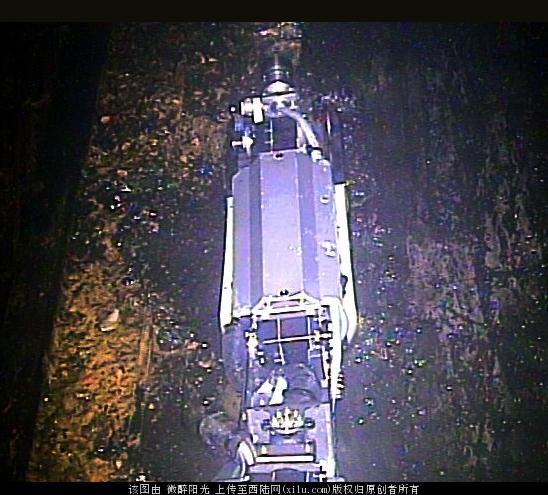
\includegraphics[width = 60mm]{../preview/Robo.jpg}
    \caption{“蝎形”("scorpion")机器人行进在福岛核电站2号反应堆内}
    \label{Robo}
\end{wrapfigure}
目前,受控无人车,即对无人车发送指令控制无人车的技术已经有了很多现实生活中的应用。然而,
这种受控无人车要求控制者能够看到无人车的运动状态,并对无人车进行控制。这样不方便无人车进一步
进行无人作业。例如,在地震灾区倒塌的房间中,控制人员无法看到无人车的具体位置,这就需要无人车
对周边环境数据进行采集,方便控制人员进行进一步的控制。另外,通过加装场地检测装置,无人车或
机器人可以到很多危险场合进行作业和信息的采集。例如,2011年日本福岛核泄漏之后,东电公司曾派遣如图
\ref{Robo}所示的机器人到反应堆内调查事故情况。通过加装摄像头和辐射监测设备,机器人可以在人类
无法承受的辐射量内进行高强度监测作业。

另外,目前3D检测和建模技术方兴未艾。利用无人机等设备对建筑物外表面进行3D检测建模的技术已经实现。
计算机视觉领域内,SfM(Shape from Motion)等基于单目摄像机的3D重建技术已经相对比较成熟,因此,
周边技术的成熟为我们的设计提供了相当的基础。同时,我们也考虑采集小车的位置信息,一方面,
对于控制人员来说,了解小车的行进路线(相对位置)也是一个很重要的信息点,另外一方面,根据计算机
的相关知识,我们也可以知道获取准确的拍摄角度和拍摄位置可以更好的加大3D重建的精度,而这方面的应用和算法
据我们所查阅的资料来看相对较少,可以进行进一步的创新。

因此我们将选题定位基于受控无人车的场地探测和3D重建系统,目标是通过控制无人车的行为,完成对场地内
图像信息的采集,并在合适的情况下允许上位机进行3D重建,完成对场景3D状态的描述工作。根据时间限制
和具体的完成情况,我们将整个项目分为如下几个部分进行。
\begin{enumerate}
    \item 第一部分
    \begin{itemize}
        \item 基本的电源管理和小车运动控制
        \item 在上位机控制下小车完成相关运动
        \item 小车安装摄像头,将图像回传上位机
    \end{itemize}
    \item 第二部分
    \begin{itemize}
        \item 图像实时回传
        \item 小车完成相对位置信息的记录和回传
        \item 利用位置信息进行二维地图的展示工作
    \end{itemize}
    \item 第三部分
    \begin{itemize}
        \item 将上位机应用部署到移动平台
        \item 小车安装避障系统,并可以自动运行
        \item 三维重建,同时利用位置信息
    \end{itemize}
\end{enumerate}
从上面我们可以看出整个工程量较大,受到两周的开发时间的限制可能不一定全部完成,剩余工程可以
作为参加挑战杯等进一步开发项目的发展方向。
\subsection{具体完成情况}
这一节总结一下提到的项目内容的完成情况

经过两周的具体调试,我们实现了第一部分的所有具体要求,包括小车的驱动模块,摄像头的安装和
测试,蓝牙模块通信的测试等,并完成了整个项目的整合。但是由于蓝牙速度较慢,经过了长时间的
调试,我们仍然不能实现图像的实时回传,同时,由于图像数据量较大,回传图像对蓝牙压力也比较大
导致蓝牙模块并不是很稳定。虽然如此,整个项目的工作量,完成度和可展示性还是非常理想的,尤其是
对基于FPGA对裸CMOS摄像头OV7670的封装等为代表的工作花费了我们大量的心血,总结起来还是比较满意的。
\section{方案比较与选择}
\subsection{主控元件的选择}
首先我们考虑主控元件的选择,根据我们的技术水平和课题的情况,可供选择的主控芯片为MCU
(单片机)和FPGA。相比FPGA,MCU具有开发相对简单的优势,以串口通信协议为例,大部分MCU
的系统库中均已经封装了串口通信协议,而FPGA相对更接近底层,因此需要自行完成相关的通信协议
的封装,这将消耗大量的时间和精力。

然而,相比于MCU,FPGA在速度和并行性方面有着很大的优势。根据我们查阅的资料,以STMF103为例,
其时钟速度可以达到72MHz,然而由于串行执行的原因,IO速度相对于FPGA较低;对比我们使用的Xilinx
FPGA,其时钟速度可以达到100MHz,同时高度并行使得模块之间互相不干扰,保证了IO速度等要求。

因此,考虑到性能要求以及课程需要,我们在硬件方面采用了FPGA作为主控进行开发。
\subsection{通信机制的选择}
根据查阅的资料,可供选择的无线通信机制有如下三种:

\begin{enumerate}
    \item WiFi信道

    这种通信机制需要将WiFi模块植入硬件,使得小车可以联网传输信息。
    上位机或移动平台使用WiFi下载信息。这种方式的优势一方面是信息传输距离较远,
    在一个路由器覆盖的范围内,信息均可以被传输。另一方面可拓展性也比较强,
    如果设计了合理的联网方式,将进一步解除距离限制,通过将信息上传到云空间,
    用户可以在任何联网的地区完成信息的收取和对小车的控制。

    这种通信机制的缺点是过于复杂,尤其是使用FPGA进行开发的情况下,网络通信协议
    将带来更大的开发时间消耗,不适用于本课程的短期开发。

    \item 蓝牙信道

    这种通信机制利用蓝牙模块,蓝牙模块已经将蓝牙信道封装成串口的形式,
    从很大程度上方便了开发。同时,通过对电脑,移动设备上的蓝牙模块进行开发,
    用户可以不依赖于第三方设备(如路由器)和小车进行通信。虽然通信速度上相比WiFi也
    有一定的损失,并且通信距离受到明显限制,但相比于WiFi模块而言,其功耗更小。

    \item SPI信道

    后期的开发表明,蓝牙的速度并不能保证摄像头传输的实时性,因此后期考虑采用SPI信道
    替代原有的蓝牙信道,然而相比于蓝牙——串口信道,SPI的开发不论是在上位机方面还是在
    FPGA方面均比较复杂,因此不一定可以完成。

\end{enumerate}
综合以上三种通信机制的优缺点,我们选择蓝牙信道作为通信手段。
\subsection{供电方式的选择}
首先通过查阅可能使用到的外设的技术手册,我们大概确定了供电需求为
\begin{itemize}
    \item 5V@1.5A
    \item 3.3V@1.5A
    \item 7.2V@40A
\end{itemize}
其中5V@1.5A负责向FPGA 5V@1A以及舵机供电,3.3V电源负责向外设供电,例如我们采用的摄像头OV7670
采用的供电电压为3.3V@100mA。7.2V@40A电源负责向电机供电,并应接受PWM调制来控制电机转速。

通过查阅资料我们发现,供电的难点在7.2V@40A电源,而5V@1.5A电源和3.3V@1.5A电源
均可以使用实验室提供的TPS54160 SMT芯片完成设计,
这一部分内容将在后面基于Webench的仿真实现上面进行说明。7.2V@40A电源的电流限额主要受到电机供电电流要求
影响,从实验室提供的数据手册我们可以发现,电机的空载电流2.4A,最高效率电流11A,堵转电流52.8A,根据网上
查阅的相关资料,电机的限流应当是最高效率电流的约4倍,因此设计7.2V@40A电源负责向电机供电。

这里讨论7.2V@40A电源的设计问题。因为需要接受PWM信号调制,因此我们采用了H桥进行设计。
\begin{wrapfigure}{r}{0pt}
    \centering
    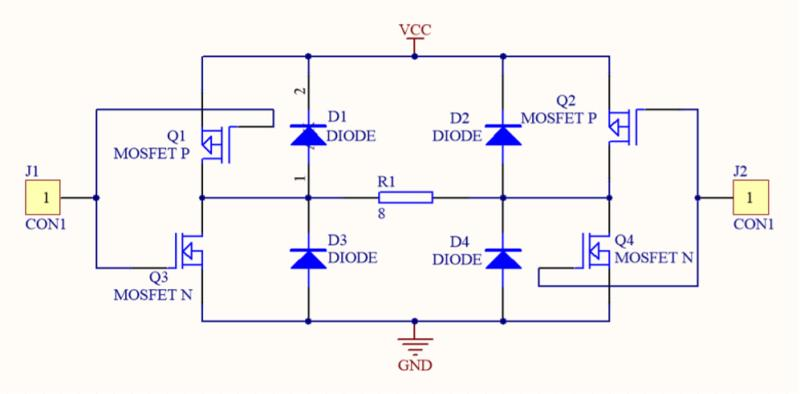
\includegraphics[width=60mm]{../preview/HBridge.jpg}
    \caption{H桥的电路原理图}
    \label{H-bridge}
\end{wrapfigure}
H桥的电路原理图如图\ref{H-bridge}所示。Q1\~Q4可以由处于饱和状态的三极管或开关状态的MOS管组成 
J1 和 J2 分别接入前一级驱动电路产生的两个反相PWM,设某时刻 J1 为高电平,
则 Q3 导通,Q1 截止;由于反相,J2 为低电平,Q2 导通,Q4 截止,
电流由通过 Q2,经负载,再经过 Q3 流入地。
同理,当某时刻 J1 为低电平时,Q1,Q4 导通, Q2,Q3 截止,
电流依次经 Q1,R1,Q4 流入地。综上,任意时刻有且只有一个对角线上的两个MOS管是导通的。

对于电机,我们可以设定刹车模式,即可以通过与上述方法类似的方法将电机两脚短路,使得电机
迅速产生电磁制动实现刹车效果

通过搜索符合要求的元件,我们发现合理的解决方案为bts7960/7961芯片和自行搭建H桥两种方案。

bts7960/7961芯片是接受5VPWM信号调制的,输入电压5.5V至27V@43A的半H桥电路,
采用SMT封装,输出电流符合要求。
然而,由于我们电机的额定输入电压为7.2V,经过对电机的初步调试我们可以发现
电机在7.2V输入电压下的转速非常高,导致速度不能得到控制,
经过进一步的实验我们发现,在低于数据手册上提供的5.4V供电的情况下,
电机的转速可以保证一个理想的状态,因此可以初步得到结论即PWM信号的占空比不可过高。

而自行搭建H桥,因为工艺比较复杂,同时在网上找不到合适的大功率MOS管供应商,
因此我们放弃了这个方案。


\subsection{摄像头数据传输技术的选择}
我们采用的OV7670摄像头,可以输出25fps 640*480 VGA格式的RGB三色图像,输出采用8线同步并行传送
因此输出时钟速度可以达到$25*640*480 \approx 8\mathrm{MHz}$。
收到蓝牙信道是串行接口的原因,蓝牙信道的速度必须达到8MB/s,这是一般蓝牙系统很难做到的。
因此不论是FPGA读取信息还是蓝牙传输信息的速度,均不如摄像头采集数据的速度,需要找到合理的解决方式。

经过我们查阅相关资料发现,OV7670的传输方式有如下三种形式:
\begin{wrapfigure}{r}{0pt}
        \centering
        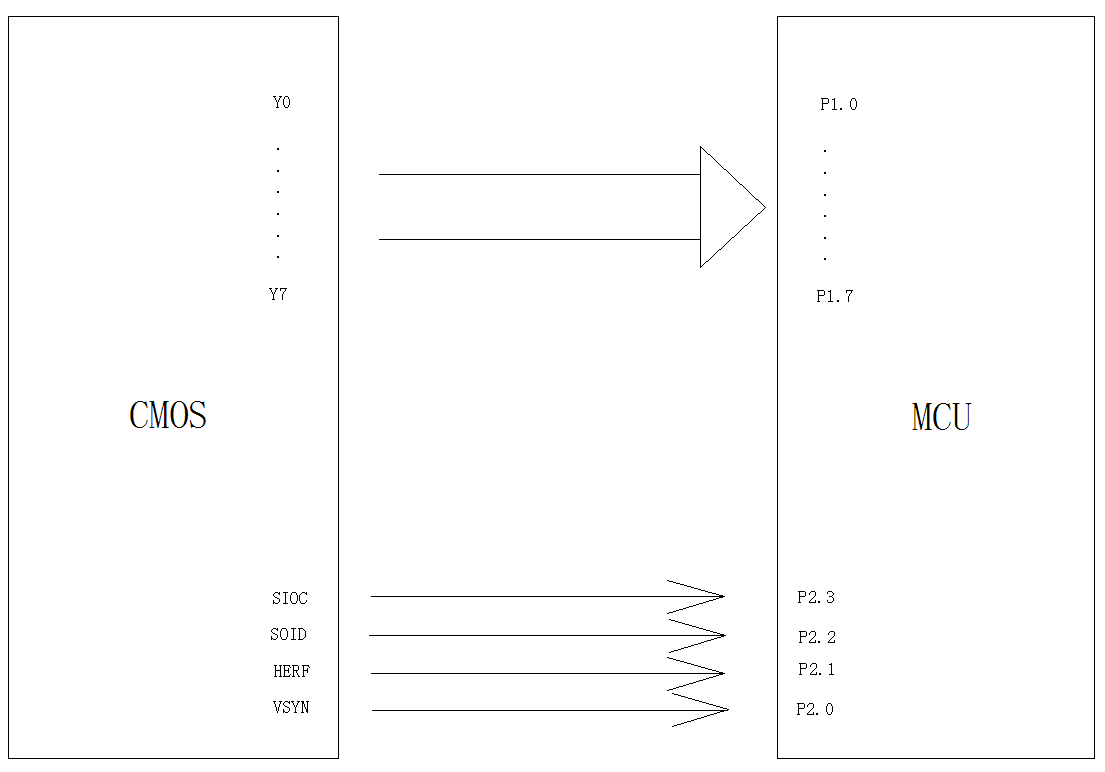
\includegraphics[width=60mm]{../preview/NFIFO.png}
        \caption{MCU/FPGA直接采集}
        \label{fig2}
        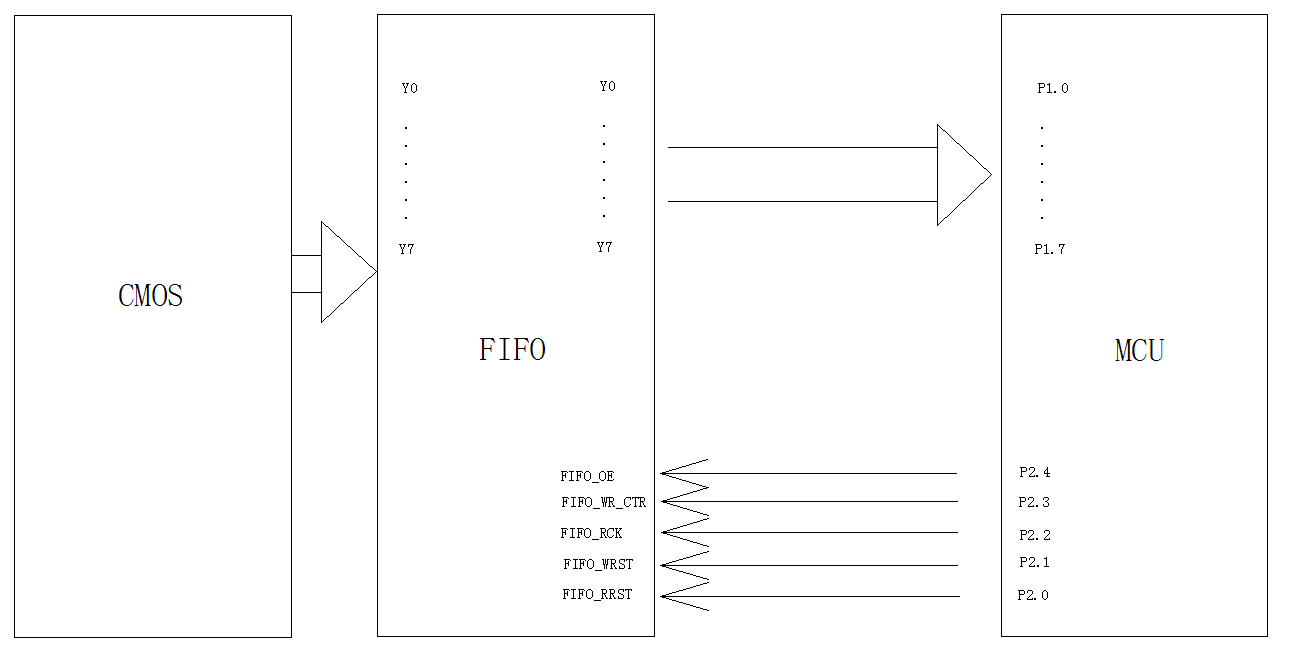
\includegraphics[width=60mm]{../preview/FIFO.png}
        \caption{FIFO采集}
        \label{fig3}
\end{wrapfigure}
\begin{itemize}
    \item MCU/FPGA直接采集:

    如图\ref{fig2}所示,这种方法是最简单,最直接,但也是最不好实现的方法,
    以MCU为例,多数的CMOS 芯片(如OV7670)的时钟速度可高达24M,
    一般MCU的IO 端口速度根本不可能达到,所以需要高速MCU。
    这对多数用户来讲有些不现实。但也不是完全没有办法在低速上实现采集,
    方法也很简单,那么就是降低CMOS的输出速度,
    不过这需要靠外部的晶振和内部的PLL电路以及像素时钟速度,
    帧速等多个寄存器共同设置,并且要和MCU的IO速度匹配才可实现。
    但这么做将带来巨大的寄存器设置工作量并导致硬件图像的采集速度
    可能下降到0.5帧以下,同时带来图像失真的可能。
\end{itemize} 

\begin{itemize}
    \item DMA方式

    这种方式主要用于MCU中,FPGA中这种方式效果不明显,DMA控制器使得数据
    可以绕过CPU直接进入内存,但是在FPGA中,同时受到串口通信速度的影响,
    这种方式效果也不是很明显。

    \item FIFO模块采集

    如图\ref{fig3},用户只需要按上述时序图控制相关的几个控制引脚即可,可以很
    方便的使用在低速MCU上,另外一个好处是,可以直接IO口读取数据,
    读出的数据可以直接送屏,也可以经过MCU简单处理;当然也可以不经过
    MCU,直接送到屏等外围器件使用。对于FPGA,以及速度相对较低的串口单元,
    使用FIFO也能很大程度的解决速度不同步的问题。

\end{itemize}
\subsection{车辆位置角度信息处理方式的选择}
为了进一步增强3D建模的精度,我们希望能够采集车辆的位置信息和角度信息。
由于摄像头和车辆是相对固定的,这样也就获得了摄像头的位置信息和角度信息。

根据我们查阅到的资料,车辆的位置信息和角度信息有几种不同的获取方式,如下所示。
\begin{itemize}
    \item 惯性测量单元(IMU)模块

    通过加速度计和陀螺仪的信息,可以直接读取车辆的加速度和角度。
    经过积分之后可以得到车辆的速度信息和角度信息,这种方法最简单,
    但是误差最大,加速度计易受到颠簸,碰撞,刹车等造成的脉冲影响,
    并进一步影响积分的准确性。角速度计(陀螺仪)具有一般性的零点迁移
    问题,这包括动态的零点波动和静态的温漂。经过积分会导致角度信息
    相当不准确。这种方法只能作为一种简单的参考,实用时必须加以处理。

    \item 磁场计

    通过对地磁角度的测定,可以直接获取车辆的角度,并通过加速度计等
    方式获得车辆的速度,这种方式误差相对前一种较小,
    但是受外界磁场的影响比较严重,尤其是当存在10A绕组的电机驱动时,
    这种方法可以认为无效。

    \item 码盘

    这种方法通过测量车辆四轮的转速经过解算得到车辆的具体位置,相比于
    之前几种方式,这种方式依赖于更加准确的光电传感器,因此得到的值也
    相对比较准确,这种方法的难点在于必须对车辆的刚性模型进行建模,
    同时安装码盘也是一个硬件上的难点。
\end{itemize}
综合提到的几种方法,我们计划采取IMU+信号处理+码盘解算几种方式
得到车辆的具体位置,希望通过反馈等方式希望得到更准确的车辆控制。

\subsection{其他注意事项}
在设计对车辆相对位置进行测量的过程中,考虑到FPGA在解算浮点数方面比较难以开发,
我们选用了NI myRIO进行解算和控制,并采用myRIO自带的WiFi进行相关数据的回传。

NI myRIO是NI针对教学和学生创新应用而最新推出的嵌入式系统开发平台。
NI myRIO内嵌Xilinx Zynq芯片,使学生可以利用双核ARM Cortex-A9的
实时性能以及Xilinx FPGA可定制化I/O,学习从简单嵌入式系统开发到
具有一定复杂度的系统设计,采用LabView语言进行可视化编程。
通过myRIO可以大幅简化控制算法如PID的调试过程,显著降低开发难度,加速开发进度。
\subsection{实际项目的修正和改动}
实际项目进行过程中,我们尽可能的对蓝牙的速度进行了利用,然而由于蓝牙速度受限,
导致实际上图像回传不能实时化,并且对蓝牙通信速度上限的冲击导致蓝牙出现不稳定情况。
在这种情况下,我们希望采用SPI-WiFi-TCP通信协议,然而TCP协议封装复杂,
经过我们查阅相关资料,TCP的引脚数量甚至超过了我们使用的FPGA的全部可控引脚数量,‘
同时TCP通信机制也比较复杂,会对是FPGA层面的封装还是上位机的编写带来巨大的困难,
因此我们最终放弃了这种思路。

同时,对于陀螺仪和测速方面,由于我们使用的FPGA引脚已经全部被占用,导致基于FPGA
的相关开发变得不现实,因此我们选用了NI myRIO进行相关的开发,并完成了陀螺仪模块。
对于测速模块,我们发现不论是车轮还是电机均很难安装码盘,因此我们采用了对车轮进行
标注并利用红外进行测速,并基于myRIO调通了相关的功能,然而由于我们设计的车辆行驶
速度偏慢,因此相关的测速变得没有实际意义,最终我们放弃了这个模块的整合工作。
\section{基于FPGA的数字系统框图}
\begin{figure}
    \centering
    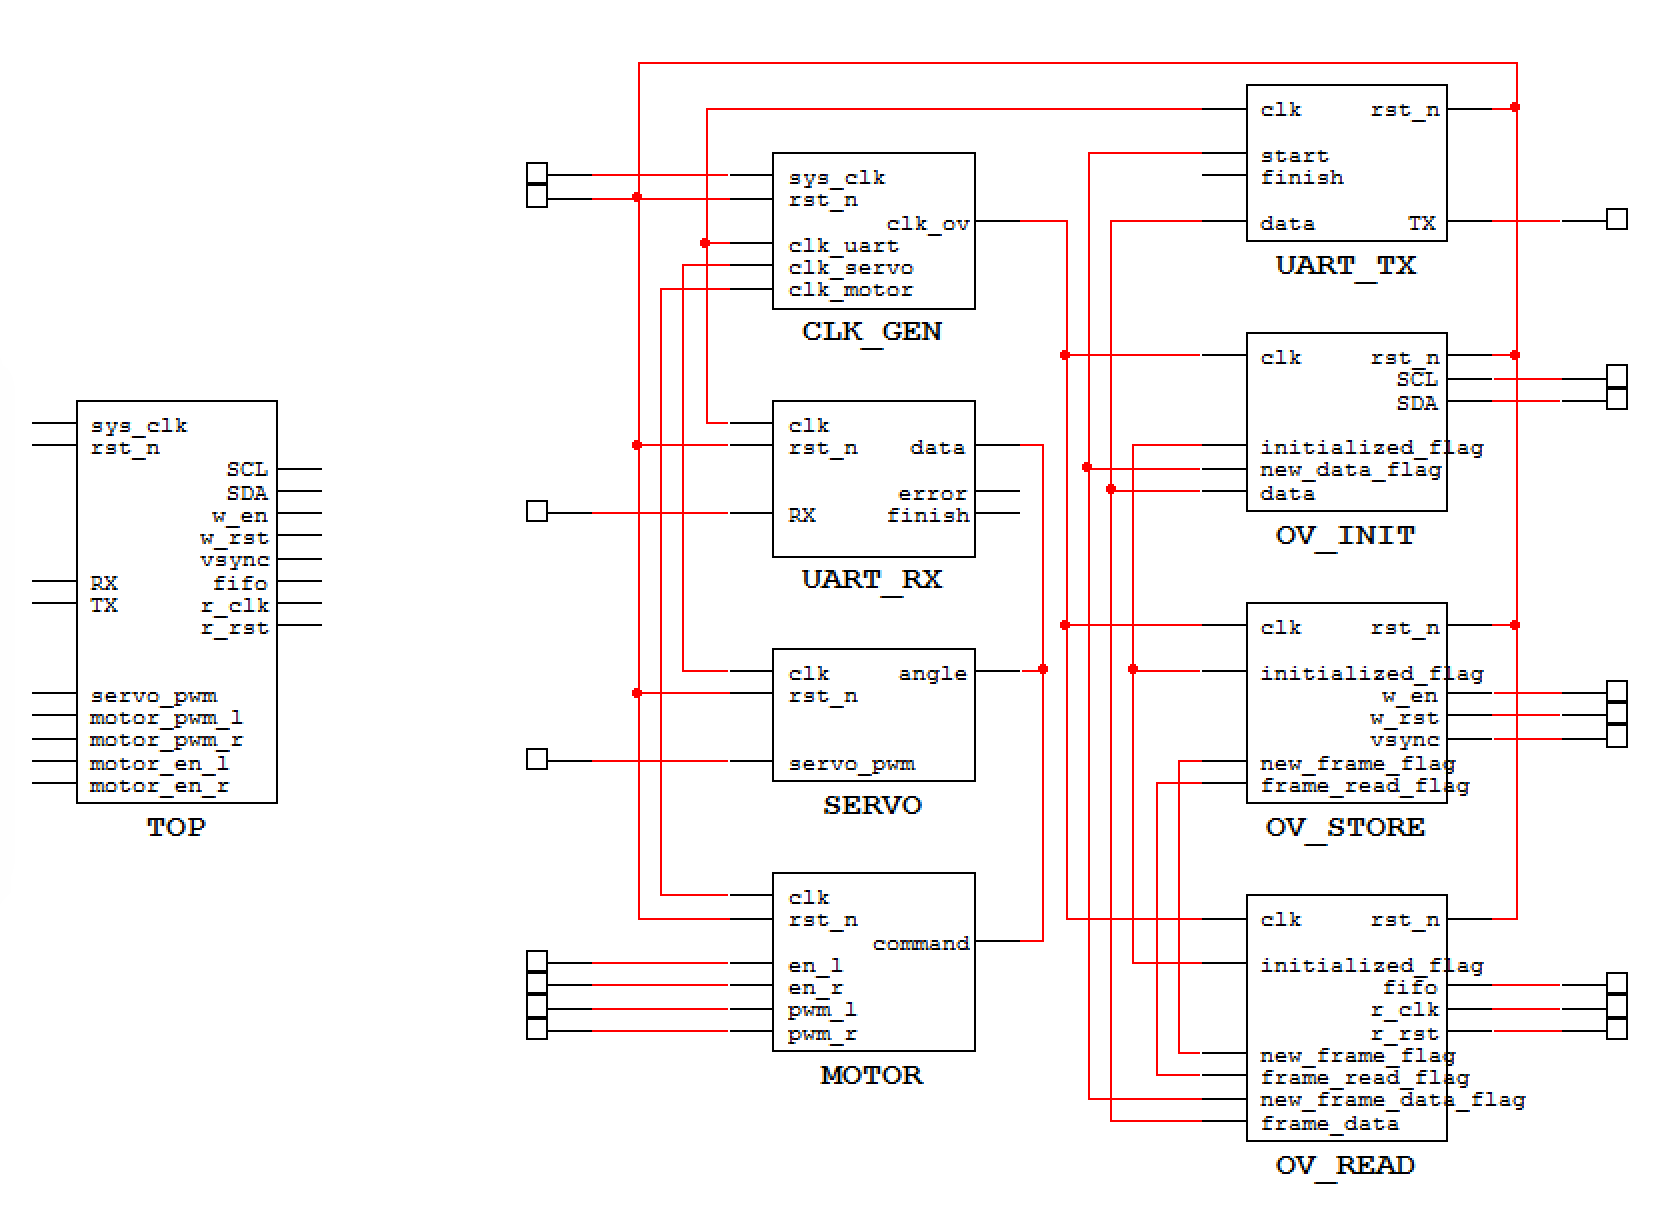
\includegraphics[width=\textwidth]{../preview/FPGABlockDesign.png}
    \caption{基于FPGA的数字系统框图}
    \label{FPGABlockDesign}
\end{figure}
如图\ref{FPGABlockDesign}所示,左侧为封装的顶层模块,从右侧可以看出共分为8个子模块。
\begin{itemize}
    \item CLK\_GEN

    该模块对100MHz系统时钟分频,输出4个时钟分别供串口、舵机、电机、摄像头使用。

    \item UART\_RX

    蓝牙串口接收模块,RX为数据线,每从上位机接收一个码元即触发finish信号,并将数据存
    在data寄存器供其他模块使用。同时内部还提供了一个error接口,接收数据发生错误时触发。

    \item UART\_TX

    蓝牙串口发送模块,TX为数据线,当触发start信号后,将data寄存器中的内容发送给上位机,
    发送完成后会得到一个finish信号反馈。

    \item SERVO

    舵机控制模块,从串口接收转向控制指令,输出舵机PWM信号。

    \item MOTOR

    电机控制模块,同样从串口接收指令,输出电机使能和PWM信号。

    \item OV\_INIT

    摄像头初始化模块,SCL和SDA为SCCB协议的时钟线和数据线,初始化前initialized\_flag为
    低电平,OV\_STORE和OV\_READ处于失能状态,初始化完成后拉高initialized\_flag,摄像头
    便可正常工作。

    \item OV\_STORE

    将摄像头采集到的图像存储于FIFO中,存储完成一帧后触发new\_frame\_flag信号,等待FPGA
    读取图像结束后才继续采集下一帧。

    \item OV\_READ

    从FIFO中读取一帧图像,并存储在frame\_data寄存器中,读取完成后触发两个信号,一个是
    frame\_read\_flag,通知摄像头可以继续采集下一帧图像,另一个是new\_frame\_data\_flag,
    通知顶层模块将读取到的数据发送给上位机。
    
\end{itemize}
\section{传感器/执行机构接口电路图}
\subsection{传感器电路}
\subsubsection{数字接口电路}
\begin{wrapfigure}{r}{0pt}
    \centering
    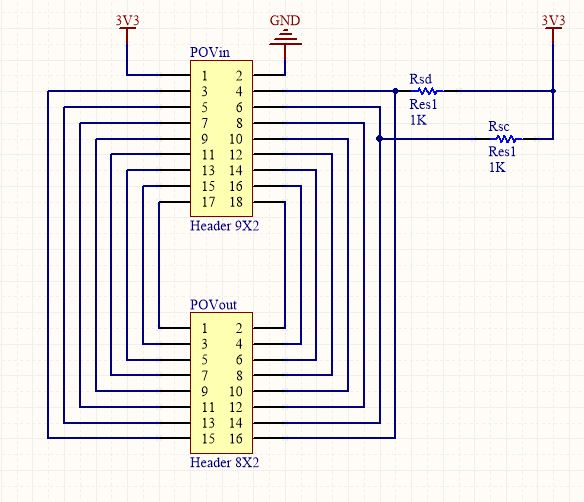
\includegraphics[width = 60mm]{../preview/ov47.jpg}
    \caption{OV上拉电阻和转接电路}
    \label{OV}
\end{wrapfigure}
这部分主要是完成数字模块之间的接口电路,由于各个数字模块已经将输出电平统一标准化为TTL电平,
因此这部分的关键主要是接口通信协议的实现,主要有FPGA方面实现了SCCB接口通信协议,串口通信协议,
摄像头数据读取协议等。另外,SIO\_C和SIO\_D分别为SCCB总线的时钟线和数据线,为了
方面对多个设备进行控制,OV的SCCB两个端口采用的均是OC门输出,需要上拉4.7k
电阻实现输出高低电平,这些需要在设计PCB的时候尽可能的考虑到并保证接线的
稳定性和摄像头位置的稳定性,因此需要在PCB上统一制作并提供对FPGA的简单的接线电路,这部分的电路
可以如图\ref{OV}所示。

\begin{wrapfigure}{r}{0pt}
    \centering
    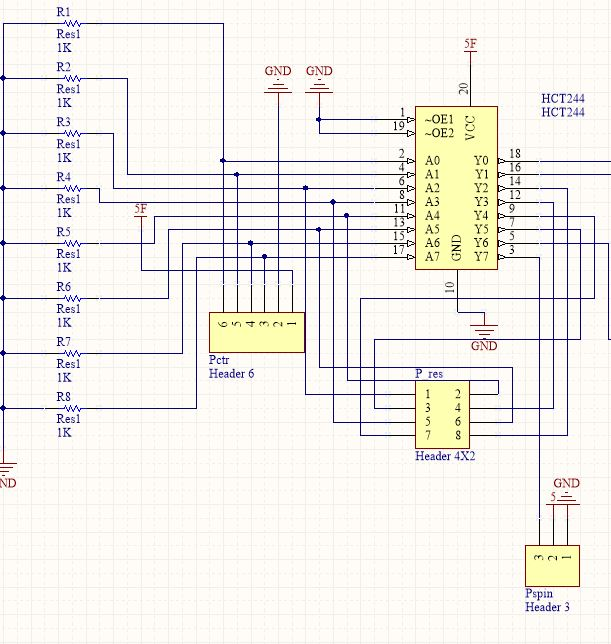
\includegraphics[width =60mm]{../preview/motor0.jpg}
    \caption{74HC244驱动器电路}
    \label{motor0}
\end{wrapfigure}
另一部分的接口电路问题是3.3V电平标准和5V电平不匹配的问题以及同时设计到的FPGA驱动能力不足的问题
通过查阅给定的技术手册我们发现FPGA输入电流1A,标准的输出电压为3.3V,
而不论是电机驱动的PWM还是舵机驱动的PWM均为5V,这中间需要设计适当的接口
电路,同时,由于工程量比较大,担心FPGA会出现总线电流过大或无法驱动相关
接口电路的情况,因此我们采用了74HC244芯片作为接口的辅助电路,74HC244是
一款高速CMOS驱动芯片,支持三态门使能,通过HC244我们可以顺利的将3.3V输出转化为5V,
并提升驱动能力。根据74HC244的接线要求,我们在输入端接入下拉电阻1k实现相关功能。这部分的电路
有如图\ref{motor0}所示。同时我们将剩下的74HC244引脚同样通过排针引出,留待之后使用。

\subsubsection{模拟接口电路}
\begin{wrapfigure}{r}{0pt}
    \centering
    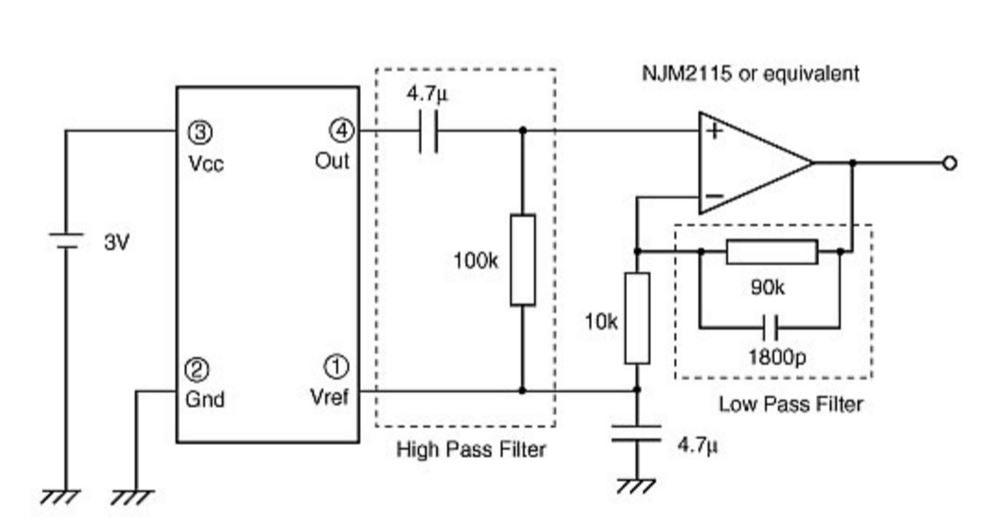
\includegraphics[width = 60mm]{../preview/enc.jpg}
    \caption{ENC-03模块外部电路图}
    \label{ENC}
\end{wrapfigure}
我们计划采用输出模拟电压的ENC-03陀螺仪,这是是一种应用科氏力原理的角速度传感器,
陀螺输出一个和角速度成正比的模拟电压信号。通过积分电路可以得到相关的角度等。根据ENC-03
技术手册,我们设计输出放大电路如图\ref{ENC}所示,整个电路由两个滤波器组成,左侧为低通滤波器,
用于滤除传感器高频噪声,右侧为高通滤波-放大电路,用于放大电压信号和滤除低频温漂。

进一步,我们搭建基本积分电路可以得到角度信息,两个信息通过AD模块可以返回给主控设备。
由于我们计划采用myRIO进行位置信息的测量,因此这部分可以直接使用LabVIEW语言在myRIO上完成,
就没有设计电路的必要了。

\subsection{执行接口电路}
这部分主要描述的是对电机和舵机的驱动电路

对于舵机驱动,单片机输出高电平为3.3V的PWM脉冲,经过前文提到过的74HC模块转5V驱动舵机旋转。

\begin{wrapfigure}{r}{0pt}
    \centering
    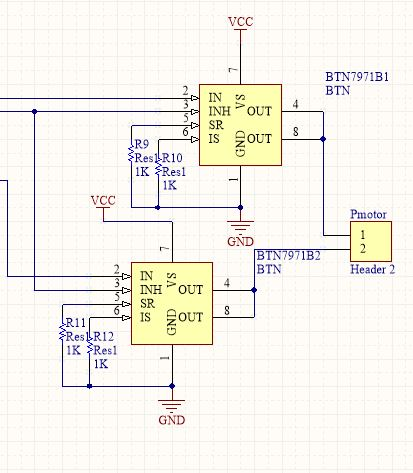
\includegraphics[width =60mm]{../preview/motor1.jpg}
    \caption{电机驱动电路}
    \label{motor1}
\end{wrapfigure}
对于电机驱动,我们使用BTN7970模块,如图\ref{motor1}所示。这里为了方便后文叙述,两片IN引脚被
命名为IN1,IN2,两片INT引脚被命名为INT1,INT2。我们将INT1,INT2短接并输入PWM波形控制电机转动速度。
将IN1,IN2分别接高低电平控制电机正转反转。例如\{INT1 = 0,INT2 = 1\}代表电机正转,\{INT1 = 1,
INT2 = 0\}代表电机反转。当\{INT1 = 0,INT2 = 0\}时,H桥全部关断,表示不控制电机转动。
当\{INT1 = 1,INT2 = 1\}时,H桥下部导通,电机两端短接,使得电机的机械能通过电磁感应和短路线
迅速释放,实现刹车功能。BTN相关引脚仍为5V接线,因此使用74HC244完成相关的电平转换和放大工作。
\section{基于Webench的电源电路仿真}
WEBENCH是TI公司提供的设计环境,通过软件工具提供定制电源等的设计,通过使用WEBENCH可以
提升设计效率。整体的设计思路如下:
\begin{itemize}
    \item 输入电压的确定

    我们将电池断开,测量电压约为8.2V,将电池直接接电机,并在电机上施加比较大的阻力,发现
    电源电压约为7V,因此我们设计电源时考虑输入电压为6V\~9V即可满足需求。

    \item 输出电压的确定

    由表\ref{t1}所示,我们需要向FPGA提供5V外接电源,对舵机提供5V外接电源,
    对外设提供3.3V外接电源,因此设计输出电压为5V,3.3V。

    \item 输出电流的确定

    首先根据实验室提供的TI样片,我们选择了TI TPS54160降压模块,TPS54160器件是一款带有集成型
    高侧MOSFET的60V,1.5A的降压稳压器。电流模式控制提供了简单外部补偿和灵活组件选择,功耗较小。

    根据TPS54160的输出电流,我们限制电源输出电流为1.5A。同时查阅技术手册可以得到主要的部件
    的供电信息如表\ref{t1}所示,总计需要输出电流5V@2A,3.3V@500mA,因此需要设计两路5V供电电源,
    其中一路FPGA自用(包括驱动器74HC244),一路给舵机/外设使用。

\end{itemize}
因此,进入WEBENCH中提供需求的输入,输出信息,选择器件为TPS54160,可以得到元件的原理图。
通过调整原理图上的元件的值的信息,可以选用已有阻值的元件进行仿真,最终确定的电路原理图和
响应时间仿真和稳态仿真如下面几张图所示。两个电路结构相同,相关参数差别如表\ref{t2}所示。
整理仿真结果如表\ref{t3}所示。可以看出电源的性能效果还是比较理想的,可以进行实际电路的搭建。
\begin{figure}
    \centering
    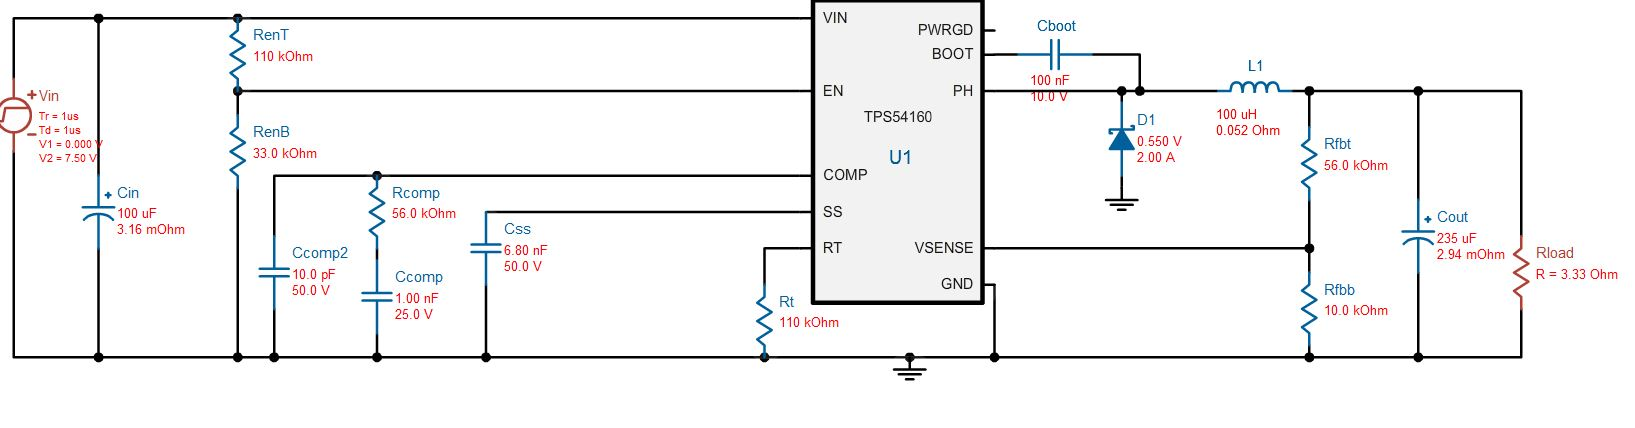
\includegraphics[width = \textwidth]{../../circuit/6-9to5V@1.5A.JPG}
\end{figure}
\begin{multicols}{2}
    \begin{table}[H]
        \centering
        \caption{主要部件供电信息}
        \label{t1}
        \begin{tabular}{|c|c|c|} \hline
            部件& 电压& 电流\\ \hline
            FPGA& 5V& 1A \\ \hline
            舵机& 5V & 800mA \\ \hline
            74HC244 & 5V& 100mA\\ \hline
            蓝牙模块 & 5V& 100mA\\ \hline
            OV7670& 3.3V& 200mA \\ \hline
        \end{tabular}
    \end{table}
    \begin{table}[H]
        \centering
        \caption{仿真主要性能指标}
        \label{t3}
        \begin{tabular}{|c|c|c|} \hline
            参数&3.3V电源&5V电源\\ \hline
            稳态电压平均值& 3.435V&5.326V\\ \hline
            稳态电压峰峰值& 3.648mV &2.465mV\\ \hline
            启动时间& 1.368ms&2.379ms\\ \hline
            电感电流峰值& 1.245A&1.753A\\ \hline
        \end{tabular}
    \end{table}
\end{multicols}
\begin{table}
    \centering
    \caption{元件参数信息}
    \label{t2}
    \begin{tabular}{|c|c|c|c|} \hline
        元件名&类别/单位& 3.3V电源& 5V电源\\ \hline
        Cin&电解电容/$\mu$F&470&470\\ \hline
        Rent&定值电阻/k$\Omega$&110&110\\ \hline
        RenB&定值电阻/k$\Omega$&33&33\\ \hline
        Ccomp&独石电容/nF&1&1\\ \hline
        Ccomp2&独石电容/pF&10&10\\ \hline
        Rcomp&定值电阻/k$\Omega$&33&56\\ \hline
        Css&独石电容/nF&6.8&6.8\\ \hline
        Rt&定值电阻/k$\Omega$&110&110\\ \hline
        Cboot&独石电容/nF&100&100\\ \hline
        D1&肖特基二极管/型号&SS24FL&SS24FL\\ \hline
        L1&定值电感/$\mu$H&100&100\\ \hline
        Rfbt&定值电阻/k$\Omega$&33&56\\ \hline
        Rfbb&定值电阻/k$\Omega$&10&10\\ \hline
        Cout&电解电容/$\mu$F&470&470\\ \hline
    \end{tabular}
\end{table}
\begin{multicols}{2}
    \begin{figure}[H]
        \centering
        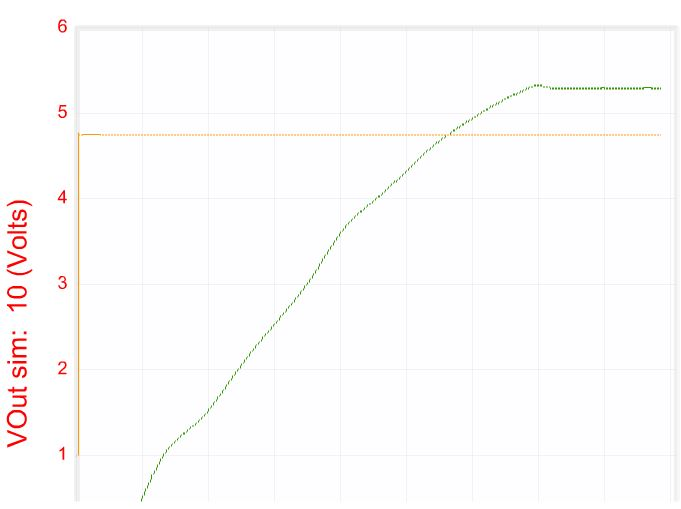
\includegraphics[width = 0.8\columnwidth]{../preview/5sim1.jpg}
        \caption{5V电源启动情况}
    \end{figure}
    \begin{figure}[H]
        \centering
        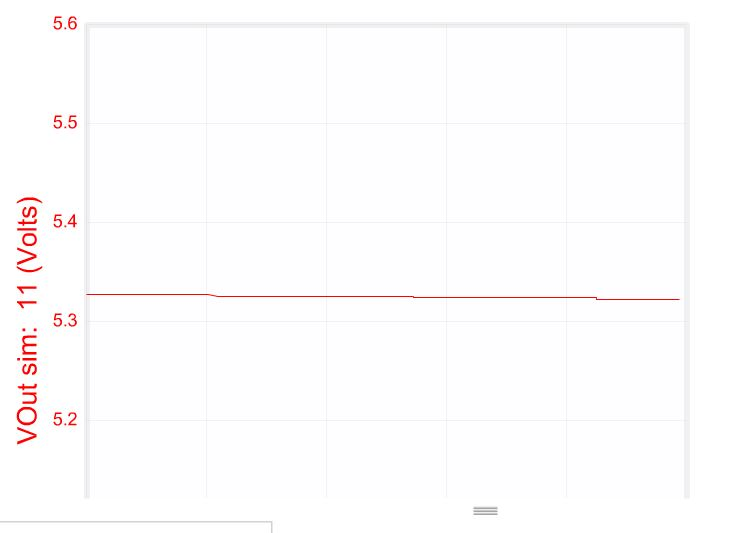
\includegraphics[width = 0.8\columnwidth]{../preview/5sim2.jpg}
        \caption{5V电源稳态情况}
    \end{figure}
    \begin{figure}[H]
        \centering
        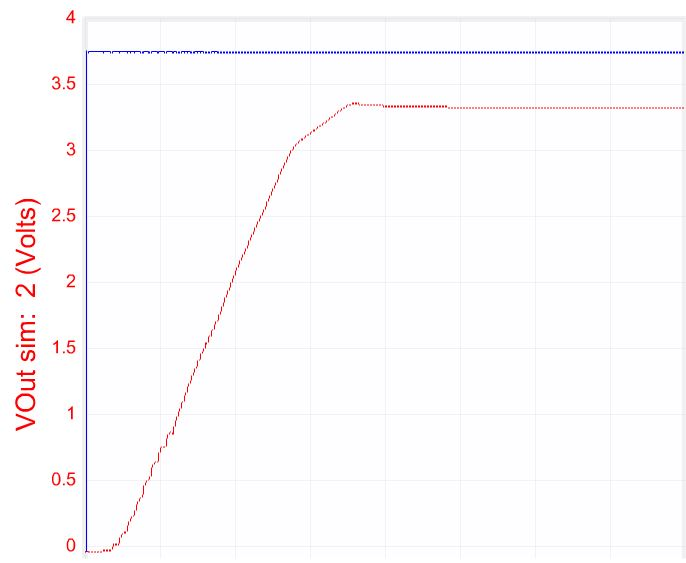
\includegraphics[width = 0.8\columnwidth]{../preview/3sim1.jpg}
        \caption{3.3V电源启动情况}
    \end{figure}
    \begin{figure}[H]
        \centering
        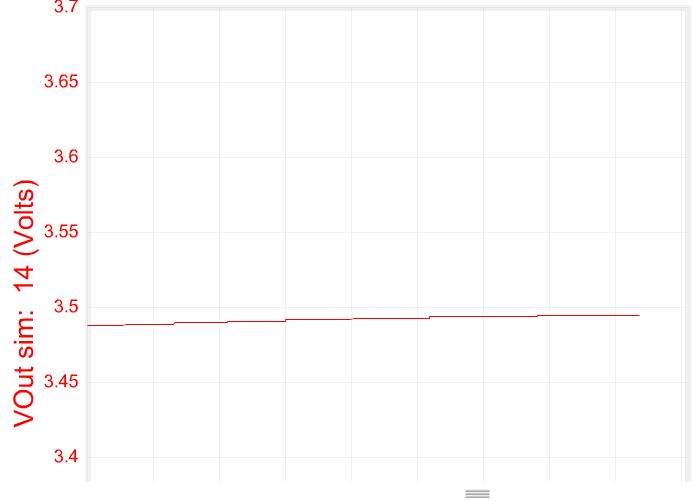
\includegraphics[width = 0.8\columnwidth]{../preview/3sim2.jpg}
        \caption{3.3V电源稳态情况}
    \end{figure}
\end{multicols}
\section{PCB的设计制作}
完成了电源模块的仿真之后就可以开始着手进行PCB的设计制作了,在设计制作的过程中,由于考虑到
手工焊接的困难,因此尽可能多的选用了插接件代替SMT封装元件,如电阻,电容等,同时,根据走线可能
涉及的电流大小如图\ref{fig4}所示,我们设计走线宽度为
\begin{itemize}
    \item 对BTN驱动板,走线40mil(1mm),对应电流3A左右
    \item 对电源管理模块,走线15mil(0.4mm),引脚处走线10mil(0.25mm),对应电流1.5A左右
\end{itemize}
同时对大电流部分加焊锡保护走线,防止过热。整版PCB单面布线,背面加装散热片,保证散热顺畅并注意
IC散热引脚接触良好。同时考虑接线端子,IC等的位置关系,充分考虑日后安装,打孔位置,
保证接线顺利同时散热合理。PCB如图\ref{pcb}所示。
\begin{table}
    \centering
    \caption{PCB线宽和电流的关系}
    \label{fig4}
    \begin{tabular}{|c|c|c|c|c|c|} \hline
        电流(A)&线宽(mm)&电流(A)&线宽(mm)\\ \hline
        6.0&2.5&5.1&2.0\\ \hline
        4.2&1.5&3.6&1.2\\ \hline
        3.3&1.0&2.8&0.8\\ \hline
        2.3&0.6&2&0.5\\ \hline
        1.7&0.4&1.3&0.3\\ \hline
        0.9&0.2&0.7&0.15\\ \hline
    \end{tabular}
\end{table}
\begin{figure}
    \centering
    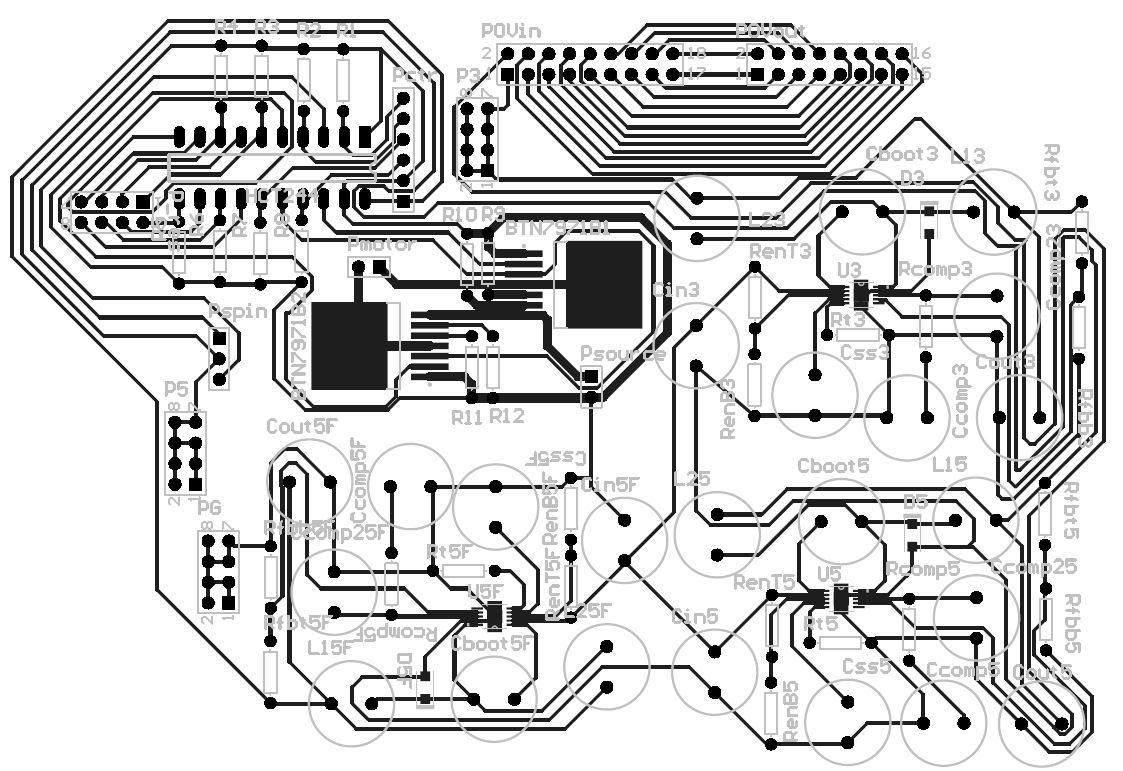
\includegraphics[width = 0.6\textwidth]{../preview/pcb_fin.jpg}
    \caption{PCB版效果图}
    \label{pcb}
\end{figure}
\section{课题开发与调试中出现的问题分析}
\subsection{数字电路部分}
% @Archer: about 100 lns?
\subsection{模拟电路部分}
\section{项目创新点}
\section{工作日志}
\section{项目完成情况}
\end{document}